\documentclass[aspectratio=169]{beamer}
\usepackage[utf8]{inputenc}
\usepackage{graphicx}
\usepackage{hyperref}

\usetheme{Madrid}
\usecolortheme{default}

% Show numeric labels [1], [2], ... in the bibliography instead of icons
\setbeamertemplate{bibliography item}{\insertbiblabel}

\title{Vision-Language Models (VLMs)}
\subtitle{Large vision-language models}
\author[Juan Irving Vasquez \textit{jivg.org}] % (optional)
{Juan Irving Vásquez\inst{1}}
\date{\today}
\titlegraphic{
\includegraphics[width=2cm]{ipn-cidetec}}

\institute[IPN] % (optional)
{
	\inst{1}%
	Centro de Innovación y Desarrollo Tecnológico en Cómputo\\
	Instituto Politécnico Nacional
}

\begin{document}
	
	% --- TITLE PAGE ---
	\begin{frame}
		\titlepage
	\end{frame}
	
	% --- INTRODUCTION ---
	\begin{frame}{What Are Vision-Language Models?}
		\begin{figure}
			\centering
			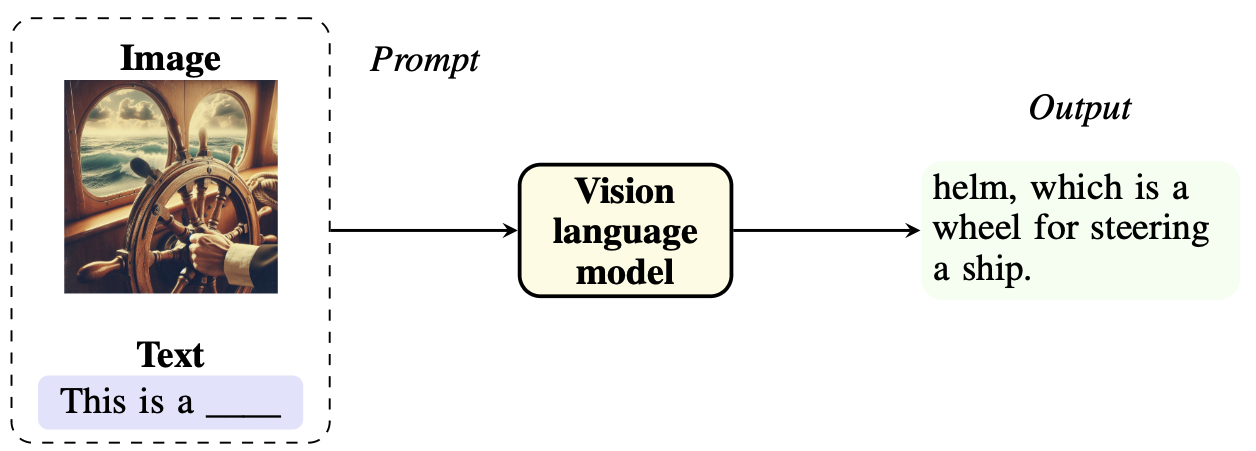
\includegraphics[width=0.6\linewidth]{vlm1.png}
			%\caption{Enter Caption}
			%\label{fig:placeholder}
		\end{figure}
		\begin{itemize}
			\item \textbf{Vision-Language Models (VLMs)} combine computer vision and natural language processing (NLP) in a single multimodal system \cite{ibm_vlm,nvidia_glossary}.
			\item They integrate a \textit{vision encoder} and a \textit{large language model (LLM)}, enabling joint reasoning over images, video, and text.
			\item Example tasks: image captioning, visual question answering, and image retrieval from text descriptions.
		\end{itemize}
	\end{frame}
	
	% --- GENERAL OVERVIEW DIAGRAM ---
	\begin{frame}{General Overview}
		\begin{figure}
			\centering
			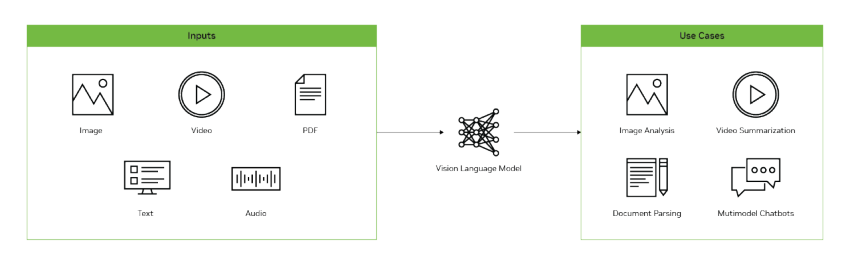
\includegraphics[width=\linewidth]{metropolis-iva-diagram-vlm-glossary-ces25-3576177-r1--1-.png}
			\caption{Example of a multimodal flow between vision and language \cite{nvidia_glossary}.}
		\end{figure}
	\end{frame}
	
	% --- IMPORTANCE ---
	\begin{frame}{Why VLMs Matter}
		\begin{itemize}
			\item They overcome the limitations of traditional vision models, since they are not restricted to a fixed set of classes or tasks.
			\item Thanks to training on large collections of image-text pairs, they can follow natural-language instructions and adapt to new tasks.
			\item They enable \textbf{multimodal generative AI} applications that integrate text, images, audio, and video.
		\end{itemize}
	\end{frame}
	
	
	% --- ARCHITECTURE (COMBINED) ---
	\begin{frame}{VLM Architecture}
		\begin{columns}[T,onlytextwidth]
			
			% --- Left column: text ---
			\begin{column}{0.45\textwidth}
				\begin{itemize}
					\item Three main building blocks:
					\begin{enumerate}
						\item \textbf{Vision encoder:} transforms images or video into embeddings.
						\item \textbf{Fusion module or projector:} aligns the vision and language spaces into a shared semantic domain.
						\item \textbf{Large language model (LLM):} interprets or generates text from the visual information.
					\end{enumerate}
					\item They are generally built on \textit{Transformer} architectures \cite{vaswani2017attention}, such as \textbf{CLIP} \cite{radford2021clip} or \textbf{ViT} \cite{dosovitskiy2021vit}.
					\item Integrating these modules enables multimodal reasoning and context-aware responses.
				\end{itemize}
			\end{column}
			
			% --- Right column: image ---
			\begin{column}{0.45\textwidth}
				\begin{figure}
					\centering
					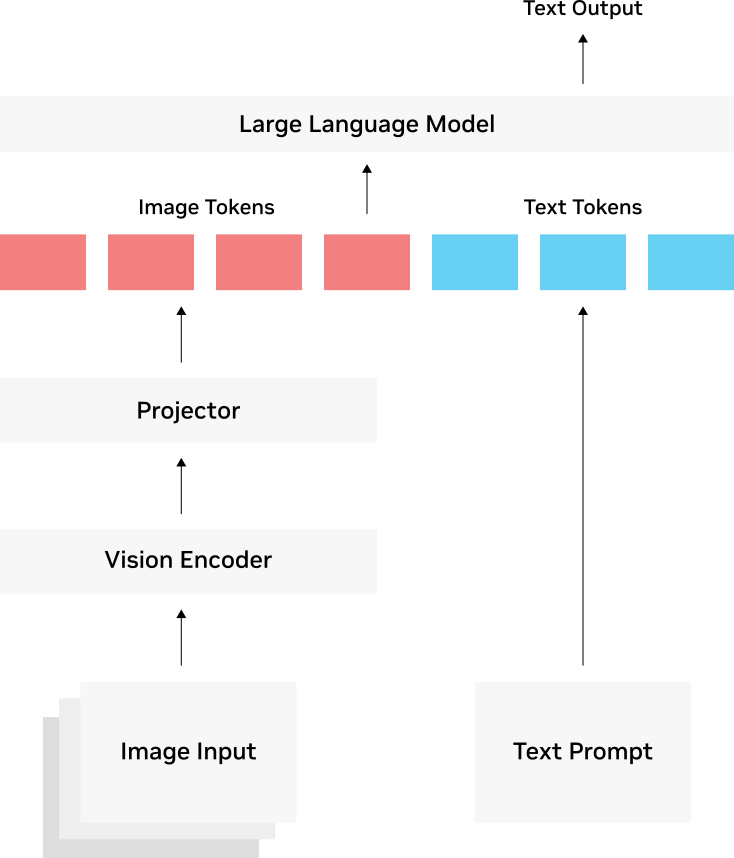
\includegraphics[width=0.7\textwidth]{vlm-architecture-diagram.png}
					\caption{Typical architecture of a vision-language model.}
				\end{figure}
			\end{column}
			
		\end{columns}
	\end{frame}
	
	
	
	% --- TRAINING ---
	\begin{frame}{Training VLMs}
		\begin{itemize}
			\item VLMs are trained using several strategies:
			\begin{enumerate}
				\item \textbf{Contrastive learning:} aligns image and text embeddings (e.g., CLIP \cite{radford2021clip}).
				\item \textbf{Masking:} predicts hidden parts of the text or image.
				\item \textbf{Generative training:} produces text from images or vice versa.
			\end{enumerate}
			\item They typically combine pretrained vision and language models before \textit{fine-tuning} on task-specific multimodal data.
		\end{itemize}
	\end{frame}
	
	\begin{frame}{Training Process Diagram}
		\begin{figure}
			\centering
			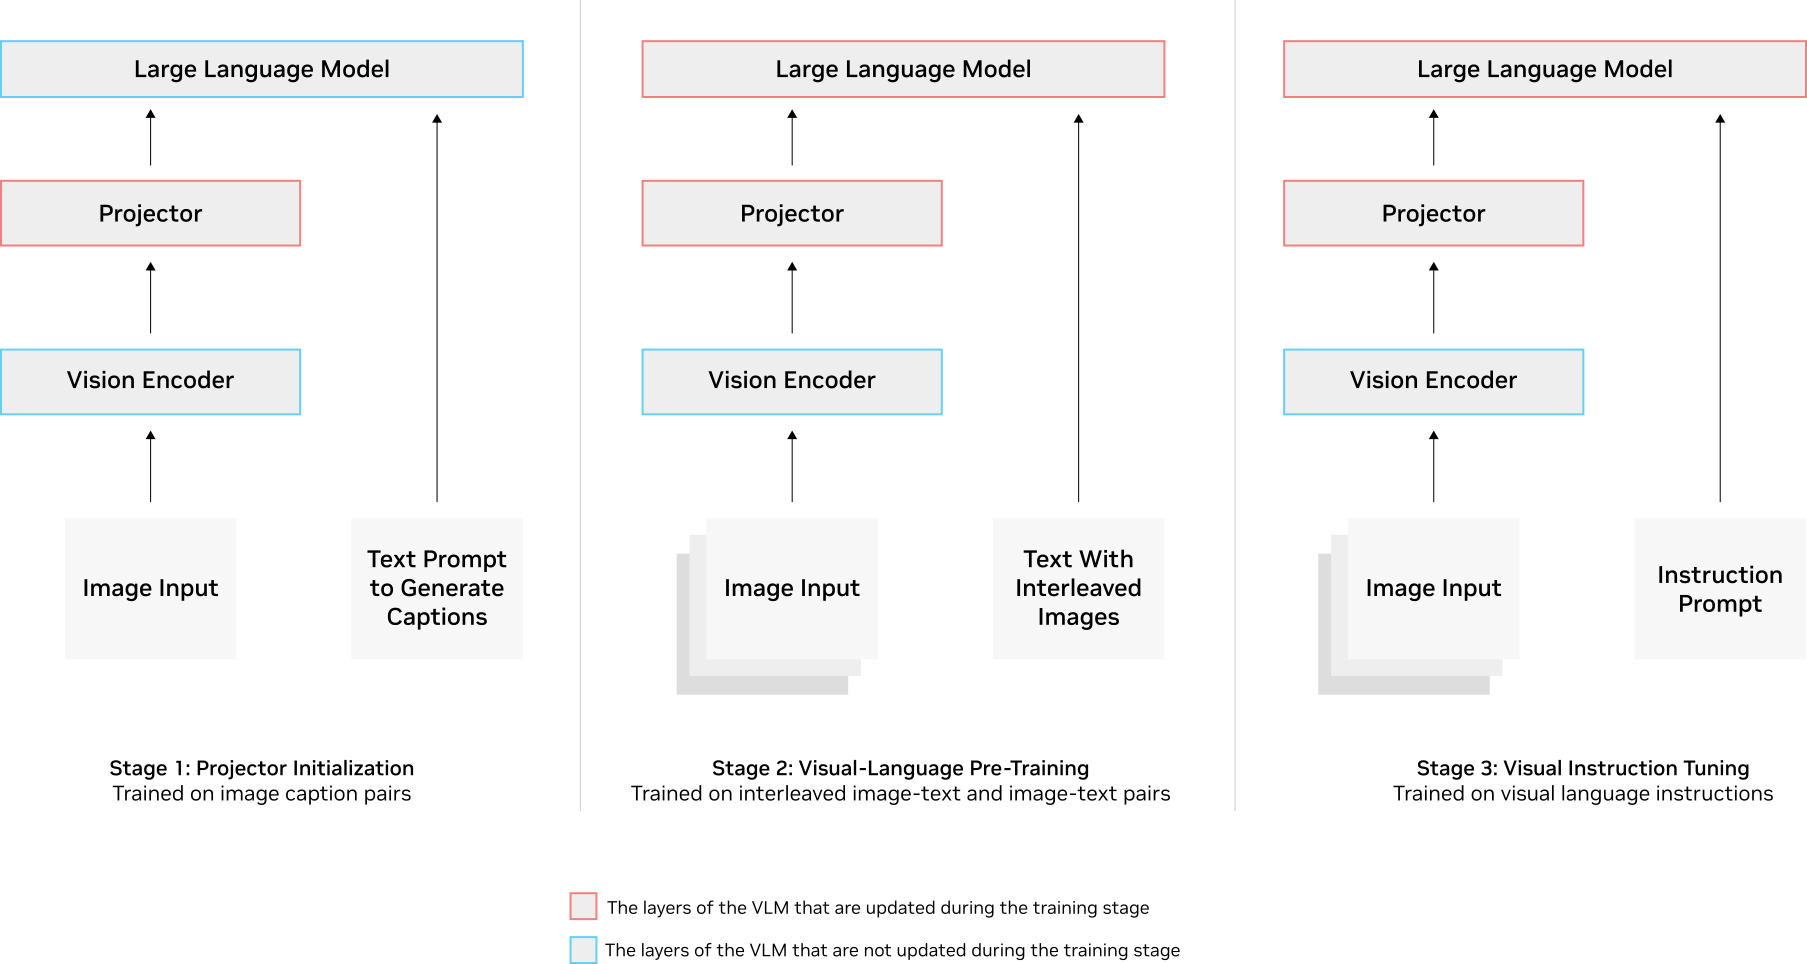
\includegraphics[width=0.9\linewidth]{vlm-training-process-diagram.png}
		\end{figure}
	\end{frame}
	
	% --- REPRESENTATIVE MODELS ---
	\begin{frame}{Representative Models}
		\begin{itemize}
			\item \textbf{CLIP (OpenAI)} \cite{radford2021clip}: pioneer of contrastive image-text learning.
			\item \textbf{GPT-4o (OpenAI)} \cite{openai2024gpt4o}: multimodal model that processes text, images, and audio.
			\item \textbf{Gemini 2.0 Flash (Google)} \cite{gemini2023,google2024gemini2}: full integration of text, images, audio, and video.
			\item \textbf{Llama 3.2 (Meta)} \cite{meta2024llama32,grattafiori2024llama3}: open model with vision and text input.
			\item \textbf{NVLM (NVIDIA)} \cite{dai2024nvlm} and \textbf{Qwen2.5-VL (Alibaba)} \cite{bai2025qwen25vl}: specialized in high-resolution images and long videos.
		\end{itemize}
	\end{frame}
	
	% --- EVALUATION ---
	\begin{frame}{Evaluating VLMs}
		\begin{itemize}
			\item VLMs are evaluated with multimodal benchmarks that measure reasoning, visual understanding, and textual accuracy:
			\begin{enumerate}
				\item \textbf{MMBench} \cite{liu2024mmbench}, \textbf{MMMU} \cite{yue2024mmmu}, \textbf{MM-Vet} \cite{yu2024mmvet}: general reasoning.
				\item \textbf{OCRBench} \cite{liu2024ocrbench}, \textbf{MathVista} \cite{lu2024mathvista}: understanding text and symbols in images.
				\item \textbf{VQA} \cite{antol2015vqa}: answering visual questions.
			\end{enumerate}
			\item Evaluation aims to measure both accuracy and the capacity for generalization and multimodal reasoning.
		\end{itemize}
	\end{frame}
	
	\begin{frame}{Evaluation Example}
		\begin{figure}
			\centering
			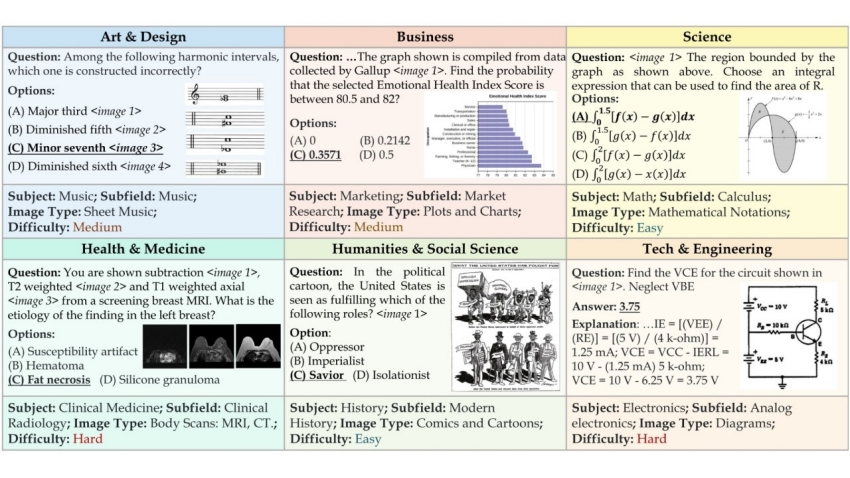
\includegraphics[width=0.8\linewidth]{vlm-mmmu-ari.jpeg}
		\end{figure}
	\end{frame}
	
	% --- APPLICATIONS ---
	\begin{frame}{Applications of VLMs}
		\begin{itemize}
			\item \textbf{Caption generation} for images or videos.
			\item \textbf{Semantic visual search}: finding images from text.
			\item \textbf{Object segmentation and detection} with textual explanations.
			\item \textbf{Visual question answering (VQA)}.
			\item \textbf{Assisted design and image generation} (text-to-image).
			\item Uses in medicine, robotics, education, art, and environmental monitoring systems.
		\end{itemize}
	\end{frame}
	
	\begin{frame}{Real-World Applications}
		\begin{figure}
			\centering
			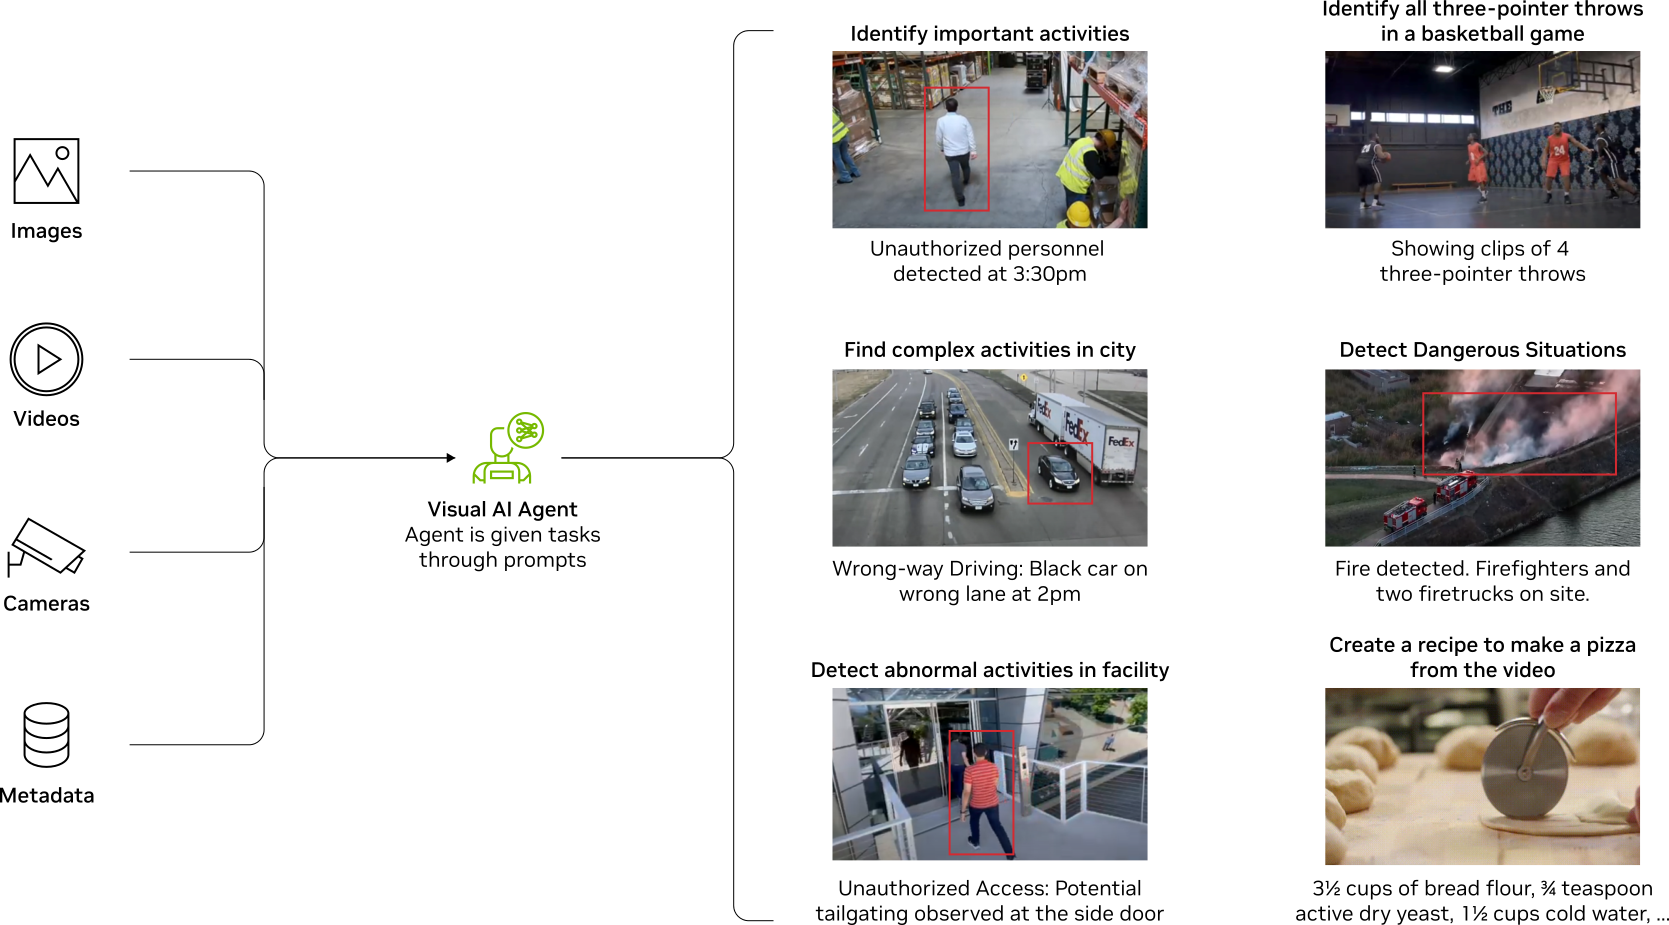
\includegraphics[width=0.8\linewidth]{vlm-real-world-diagram.png}
		\end{figure}
	\end{frame}
	
	% --- CHALLENGES ---
	\begin{frame}{Challenges and Risks}
		\begin{itemize}
			\item \textbf{Data bias:} models may reflect prejudices present in the training sets.
			\item \textbf{High computational costs} for training and deployment.
			\item \textbf{Limited generalization} to unseen or out-of-domain scenarios.
			\item \textbf{Hallucinations}: generating false or incorrect descriptions.
			\item \textbf{Governance and ethics}: the need for regulation, validation, and human oversight.
		\end{itemize}
	\end{frame}
	
	% --- CONCLUSIONS ---
	\begin{frame}{Conclusions}
		\begin{itemize}
			\item VLMs integrate visual and linguistic understanding in a single system, enabling a new generation of multimodal applications.
			\item They represent a step toward \textbf{generalist AI}, capable of reasoning across multiple modalities.
			\item Their future depends on advances in alignment, ethics, efficiency, and robustness.
		\end{itemize}
	\end{frame}
	
	% --- REFERENCES ---
	\begin{frame}[allowframebreaks]{References}
		\scriptsize
		\begin{thebibliography}{99}
			
			% --- Overviews ---
			\bibitem{ibm_vlm} IBM Think (2025). \textit{What are Vision-Language Models?} Available at: \url{https://www.ibm.com/think/topics/vision-language-models}
			
			\bibitem{nvidia_glossary} NVIDIA Glossary (2024). \textit{What are Vision-Language Models?} Available at: \url{https://www.nvidia.com/en-us/glossary/vision-language-models/}
			
			% --- Architectures ---
			\bibitem{vaswani2017attention} A. Vaswani, N. Shazeer, N. Parmar, J. Uszkoreit, L. Jones, A. N. Gomez, Ł. Kaiser, and I. Polosukhin (2017). Attention Is All You Need. In \textit{Advances in Neural Information Processing Systems (NeurIPS)}, 30.
			
			\bibitem{radford2021clip} A. Radford, J. W. Kim, C. Hallacy, A. Ramesh, G. Goh, S. Agarwal, G. Sastry, A. Askell, P. Mishkin, J. Clark, G. Krueger, and I. Sutskever (2021). Learning Transferable Visual Models From Natural Language Supervision. In \textit{Proceedings of the 38th International Conference on Machine Learning (ICML)}, PMLR 139, pp. 8748--8763.
			
			\bibitem{dosovitskiy2021vit} A. Dosovitskiy, L. Beyer, A. Kolesnikov, D. Weissenborn, X. Zhai, T. Unterthiner, M. Dehghani, M. Minderer, G. Heigold, S. Gelly, J. Uszkoreit, and N. Houlsby (2021). An Image is Worth 16x16 Words: Transformers for Image Recognition at Scale. In \textit{International Conference on Learning Representations (ICLR)}.
			
			% --- Models ---
			\bibitem{openai2024gpt4o} OpenAI (2024). GPT-4o System Card. \textit{arXiv preprint arXiv:2410.21276}.
			
			\bibitem{gemini2023} Gemini Team, Google (2023). Gemini: A Family of Highly Capable Multimodal Models. \textit{arXiv preprint arXiv:2312.11805}.
			
			\bibitem{google2024gemini2} S. Pichai, D. Hassabis, and K. Kavukcuoglu (2024). Introducing Gemini 2.0: our new AI model for the agentic era. \textit{Google Blog}. Available at: \url{https://blog.google/technology/google-deepmind/google-gemini-ai-update-december-2024/}
			
			\bibitem{meta2024llama32} Meta AI (2024). Llama 3.2: Revolutionizing edge AI and vision with open, customizable models. Available at: \url{https://ai.meta.com/blog/llama-3-2-connect-2024-vision-edge-mobile-devices/}
			
			\bibitem{grattafiori2024llama3} A. Grattafiori, A. Dubey, A. Jauhri, et al. (2024). The Llama 3 Herd of Models. \textit{arXiv preprint arXiv:2407.21783}.
			
			\bibitem{dai2024nvlm} W. Dai, N. Lee, B. Wang, Z. Yang, Z. Liu, J. Barker, T. Rintamaki, M. Shoeybi, B. Catanzaro, and W. Ping (2024). NVLM: Open Frontier-Class Multimodal LLMs. \textit{arXiv preprint arXiv:2409.11402}.
			
			\bibitem{bai2025qwen25vl} S. Bai, K. Chen, X. Liu, J. Wang, W. Ge, S. Song, K. Dang, P. Wang, S. Wang, J. Tang, et al. (2025). Qwen2.5-VL Technical Report. \textit{arXiv preprint arXiv:2502.13923}.
			
			% --- Benchmarks ---
			\bibitem{liu2024mmbench} Y. Liu, H. Duan, Y. Zhang, B. Li, S. Zhang, W. Zhao, Y. Yuan, J. Wang, C. He, Z. Liu, K. Chen, and D. Lin (2024). MMBench: Is Your Multi-modal Model an All-around Player? In \textit{European Conference on Computer Vision (ECCV)}, pp. 216--233.
			
			\bibitem{yue2024mmmu} X. Yue, Y. Ni, K. Zhang, T. Zheng, R. Liu, G. Zhang, S. Stevens, D. Jiang, W. Ren, Y. Sun, et al. (2024). MMMU: A Massive Multi-discipline Multimodal Understanding and Reasoning Benchmark for Expert AGI. In \textit{Proceedings of the IEEE/CVF Conference on Computer Vision and Pattern Recognition (CVPR)}, pp. 9556--9567.
			
			\bibitem{yu2024mmvet} W. Yu, Z. Yang, L. Li, J. Wang, K. Lin, Z. Liu, X. Wang, and L. Wang (2024). MM-Vet: Evaluating Large Multimodal Models for Integrated Capabilities. In \textit{Proceedings of the 41st International Conference on Machine Learning (ICML)}, PMLR 235.
			
			\bibitem{liu2024ocrbench} Y. Liu, Z. Li, M. Huang, B. Yang, W. Yu, C. Li, X.-C. Yin, C.-L. Liu, L. Jin, and X. Bai (2024). OCRBench: On the Hidden Mystery of OCR in Large Multimodal Models. \textit{Science China Information Sciences}, 67(12), 220102.
			
			\bibitem{lu2024mathvista} P. Lu, H. Bansal, T. Xia, J. Liu, C. Li, H. Hajishirzi, H. Cheng, K.-W. Chang, M. Galley, and J. Gao (2024). MathVista: Evaluating Mathematical Reasoning of Foundation Models in Visual Contexts. In \textit{International Conference on Learning Representations (ICLR)}.
			
			\bibitem{antol2015vqa} S. Antol, A. Agrawal, J. Lu, M. Mitchell, D. Batra, C. L. Zitnick, and D. Parikh (2015). VQA: Visual Question Answering. In \textit{Proceedings of the IEEE International Conference on Computer Vision (ICCV)}, pp. 2425--2433.
			
		\end{thebibliography}
	\end{frame}
	
\end{document}